\documentclass[aspectratio=169,10pt]{beamer}

\usepackage[T1]{fontenc}
\usepackage[utf8]{inputenc}
\usepackage[spanish,es-noshorthands,es-tabla]{babel}
\usepackage{graphicx}
\graphicspath{{capturas/}{Billing/capturas/}}
\usepackage{listings}
\usepackage{xcolor}
\usepackage{tikz}
\usetikzlibrary{shapes,arrows,positioning,calc}
\usepackage{tcolorbox}
\tcbuselibrary{skins,listings}
\usepackage{tabularx}
\usepackage{array}

% Colores de la paleta Obsidian & Pro (Estilo Anti-AI Profesional de Alta Gama)
\definecolor{bgdark}{HTML}{0B1120}
\definecolor{cardbg}{HTML}{131D33}
\definecolor{accentblue}{HTML}{38BDF8}
\definecolor{accentgreen}{HTML}{34D399}
\definecolor{accentamber}{HTML}{FBBF24}
\definecolor{accentred}{HTML}{F87171}
\definecolor{textwhite}{HTML}{F8FAFC}
\definecolor{textgray}{HTML}{94A3B8}
\definecolor{codebg}{HTML}{0F172A}
\definecolor{tableheader}{HTML}{1E293B}

% Configuración global de Beamer
\setbeamercolor{background canvas}{bg=bgdark}
\setbeamercolor{normal text}{fg=textwhite}
\setbeamercolor{title}{fg=accentblue}
\setbeamercolor{frametitle}{fg=accentblue}
\setbeamerfont{frametitle}{series=\bfseries,size=\large}
\setbeamertemplate{navigation symbols}{}

% Pie de página personalizado sin desbordamientos
\setbeamertemplate{footline}{
    \leavevmode%
    \hbox{%
    \begin{beamercolorbox}[wd=\paperwidth,ht=2.4ex,dp=0.8ex,leftskip=0.8cm,rightskip=0.8cm]{normal text}%
        \fontsize{5.8pt}{6.8pt}\selectfont\color{textgray}
        Sistema de Facturación SUNAT UBL 2.1 \quad $\bullet$ \quad Automatización con PHPUnit 10.5
        \hfill
        \insertframenumber{} / \inserttotalframenumber
    \end{beamercolorbox}}%
    \vskip0pt%
}

% Configuración de Listings para código PHP 8
\lstdefinelanguage{PHP8}{
    keywords={class, public, private, protected, function, return, new, throws, namespace, use, void, extends, static, const, false, true, null, int, string, float, array, bool, match, throw},
    keywordstyle=\color{accentblue}\bfseries,
    morekeywords={DataProvider, Test, Depends, Override},
    sensitive=true,
    comment=[l]{//},
    morecomment=[s]{/*}{*/},
    commentstyle=\color{textgray}\itshape,
    stringstyle=\color{accentgreen},
    morestring=[b]',
    morestring=[b]"
}

\lstset{
    language=PHP8,
    basicstyle=\fontsize{4.9pt}{5.9pt}\fontfamily{pcr}\selectfont\color{textwhite},
    numbers=left,
    numberstyle=\fontsize{4.2pt}{5.2pt}\selectfont\color{textgray},
    stepnumber=1,
    numbersep=4pt,
    backgroundcolor=\color{cardbg},
    showspaces=false,
    showstringspaces=false,
    showtabs=false,
    frame=none,
    tabsize=2,
    breaklines=true,
    breakatwhitespace=false
}

% Cajas tcolorbox con padding milimétrico anti-desbordamiento
\tcbset{
    colupper=textwhite,
    collower=textwhite,
    boxrule=0mm,
    arc=2mm,
    left=2.5mm,
    right=2mm,
    top=2mm,
    bottom=2mm,
    fontupper=\fontsize{6.8pt}{8.2pt}\selectfont
}

% Ventana macOS de código (botones rojo, amarillo, verde)
\newtcolorbox{codebox}[2][]{
    enhanced,
    colback=cardbg,
    colframe=cardbg,
    arc=2.5mm,
    boxrule=0mm,
    left=3mm,
    right=2mm,
    top=3.5mm,
    bottom=2mm,
    overlay={
        \fill[accentred] ([xshift=3.5mm, yshift=-2.2mm]frame.north west) circle (0.85mm);
        \fill[accentamber] ([xshift=6.5mm, yshift=-2.2mm]frame.north west) circle (0.85mm);
        \fill[accentgreen] ([xshift=9.5mm, yshift=-2.2mm]frame.north west) circle (0.85mm);
        \node[anchor=north, font=\fontsize{5.5pt}{6.5pt}\fontfamily{pcr}\selectfont\color{textgray}] at ([yshift=-1mm]frame.north) {#2};
    },
    #1
}

\begin{document}

% ==========================================
% SLIDE 1: PORTADA OFICIAL
% ==========================================
\begin{frame}[plain]
\vspace{0.6cm}
\begin{center}
    {\fontsize{7.5pt}{8.5pt}\selectfont\bfseries\color{accentblue}UNIVERSIDAD NACIONAL DE INGENIERÍA \quad $\bullet$ \quad FACULTAD DE SISTEMAS}\\[0.1cm]
    {\fontsize{6.8pt}{7.8pt}\selectfont\color{textgray}CURSO: PRUEBAS Y ASEGURAMIENTO DE LA CALIDAD DE SOFTWARE (QA)}\\[0.4cm]

    {\fontsize{14pt}{16pt}\selectfont\bfseries\color{textwhite}Automatización de Pruebas de Software con PHPUnit 10.5}\\[0.15cm]
    {\fontsize{9pt}{10.5pt}\selectfont\color{accentblue}Auditoría y Certificación del Sistema de Facturación Electrónica SUNAT UBL 2.1}\\[0.45cm]

    \begin{tcolorbox}[colback=cardbg, colframe=cardbg, width=0.88\textwidth, arc=2.5mm, boxrule=0mm, top=3mm, bottom=3mm]
        \begin{center}
        \fontsize{7.5pt}{9.5pt}\selectfont\bfseries\color{accentamber}INTEGRANTES DEL EQUIPO:\\[0.12cm]
        \color{textwhite}
        Apolinario Rodriguez, Luis Fernando \quad $\bullet$ \quad Umeres Vilca, Gustavo Aron\\[0.06cm]
        Vasquez Falcón, Mariana Ysabel \quad $\bullet$ \quad Ventocilla Alcantara, Alessandro Tito
        \end{center}
    \end{tcolorbox}
    \vspace{0.25cm}
    {\fontsize{6.2pt}{7.2pt}\selectfont\color{textgray}Lima, Perú \quad $\bullet$ \quad Repositorio: \texttt{github.com/fujimor1/Billing}}
\end{center}
\end{frame}

% ==========================================
% SLIDE 2: QUÉ ES PHPUNIT Y EL FRAMEWORK
% ==========================================
\begin{frame}{1. ¿Qué es PHPUnit y por qué lo usamos?}
\begin{columns}
\begin{column}{0.48\textwidth}
    \begin{tcolorbox}[colback=cardbg, colframe=cardbg, title=\color{accentblue}\bfseries El Estándar Global de la Industria]
        \textbf{PHPUnit} es el framework oficial de pruebas unitarias en PHP, creado por Sebastian Bergmann sobre el estándar xUnit de Kent Beck.
        \begin{itemize}
            \item \textbf{PHPUnit 10.5:} Arquitectura con tipado estricto (\texttt{declare(strict\_types=1)}), soporte para PHP 8.2 y 8.3.
            \item \textbf{Cero dependencias externas:} Ejecuta la suite directamente en RAM (CLI autónomo).
            \item \textbf{Orquestación XML:} Gestionado vía \texttt{phpunit.xml} para aislar suites, controlar advertencias y generar informes.
        \end{itemize}
    \end{tcolorbox}
\end{column}
\begin{column}{0.52\textwidth}
    \begin{tcolorbox}[colback=cardbg, colframe=cardbg, title=\color{accentgreen}\bfseries Arquitectura del Runner de Pruebas]
        \textbf{¿Cómo garantiza la rigurosidad fiscal?}
        \begin{itemize}
            \item \textbf{Test Runner:} Carga dinámicamente las clases que heredan de \texttt{TestCase} y las aísla por proceso.
            \item \textbf{Flags de Calidad Innegociables:}
            \begin{itemize}
                \item \texttt{failOnWarning="true"}: Ninguna advertencia es tolerada.
                \item \texttt{failOnRisky="true"}: Tests sin aserciones se marcan como fallos.
                \item \texttt{beStrictAboutOutputDuringTests="true"}: Prohíbe cualquier \texttt{echo} o fuga de salida.
            \end{itemize}
        \end{itemize}
    \end{tcolorbox}
\end{column}
\end{columns}
\end{frame}

% ==========================================
% SLIDE 3: CICLO DE VIDA DE LAS PRUEBAS
% ==========================================
\begin{frame}[fragile]{2. El Ciclo de Vida de las Pruebas (Test Lifecycle)}
\begin{columns}
\begin{column}{0.48\textwidth}
    \begin{tcolorbox}[colback=cardbg, colframe=cardbg, title=\color{accentamber}\bfseries Aislamiento Atómico por Caso de Prueba]
        Cada método \texttt{test*()} se ejecuta en una instancia completamente limpia e independiente:
        \begin{enumerate}
            \item \textbf{setUp():} Se ejecuta \textbf{antes} de cada test. Crea la base de datos SQLite en memoria e inicializa el catálogo.
            \item \textbf{testMethod():} Ejecuta la lógica del caso de prueba y valida las aserciones.
            \item \textbf{tearDown():} Se ejecuta \textbf{después} de cada test. Cierra conexiones y destruye el estado volátil.
        \end{enumerate}
        \vspace{0.05cm}
        \textbf{Invariante:} Un fallo en un test jamás contamina las pruebas posteriores.
    \end{tcolorbox}
\end{column}
\begin{column}{0.52\textwidth}
    \begin{codebox}{tests/Integration/SqlitePersistenceTest.php}
\begin{lstlisting}
class SqlitePersistenceTest extends TestCase 
{
    private PDO $db;

    // 1. ANTES DE CADA TEST: Inicializacion limpia
    protected function setUp(): void 
    {
        $this->db = new PDO('sqlite::memory:');
        $this->db->setAttribute(
            PDO::ATTR_ERRMODE, 
            PDO::ERRMODE_EXCEPTION
        );
        $this->crearTablasYSembrarCatalogo();
    }

    // 2. DESPUES DE CADA TEST: Destruccion de recursos
    protected function tearDown(): void 
    {
        unset($this->db);
    }
}
\end{lstlisting}
    \end{codebox}
\end{column}
\end{columns}
\end{frame}

% ==========================================
% SLIDE 4: PATRÓN AAA Y PRINCIPIOS FIRST
% ==========================================
\begin{frame}[fragile]{3. El Patrón AAA (Arrange - Act - Assert) \& Principios FIRST}
\begin{columns}
\begin{column}{0.48\textwidth}
    \begin{tcolorbox}[colback=cardbg, colframe=cardbg, title=\color{accentblue}\bfseries Estructura Canónica AAA]
        Cada prueba sigue estrictamente las tres etapas:
        \begin{itemize}
            \item \textbf{Arrange (Preparar):} Instanciar los Value Objects, configurar el emisor y el estado inicial.
            \item \textbf{Act (Actuar):} Invocar la operación del dominio (ej. \texttt{crearFactura()}).
            \item \textbf{Assert (Verificar):} Comprobar que los resultados coincidan con el estándar tributario.
        \end{itemize}
    \end{tcolorbox}
    \vspace{0.1cm}
    \begin{tcolorbox}[colback=cardbg, colframe=cardbg, title=\color{accentgreen}\bfseries Principios FIRST de Robert C. Martin]
        \textbf{Fast:} 39 pruebas en 0.21s $\bullet$ \textbf{Independent:} Cero acoplamiento $\bullet$ \textbf{Repeatable:} Mismo resultado $\bullet$ \textbf{Self-validating:} Pasa o Falla $\bullet$ \textbf{Timely:} TDD.
    \end{tcolorbox}
\end{column}
\begin{column}{0.52\textwidth}
    \begin{codebox}{tests/Unit/ComprobanteTest.php}
\begin{lstlisting}
public function testEmiteFacturaValidaConIgv(): void 
{
    // 1. ARRANGE: Preparamos entidades del dominio
    $emisor  = new Emisor(new Ruc('20131312955'));
    $cliente = new Cliente(new Ruc('20100047218'));
    $item    = new Detalle('Laptop', 2000.0, 1, '10');

    // 2. ACT: Ejecutamos la regla de negocio
    $factura = Comprobante::crearFactura(
        'F001', 1, $emisor, $cliente, [$item]
    );

    // 3. ASSERT: Comprobamos liquidacion exacta
    $this->assertSame(2000.0, $factura->getSubtotal());
    $this->assertSame(360.0,  $factura->getIgv());
    $this->assertSame(2360.0, $factura->getTotal());
}
\end{lstlisting}
    \end{codebox}
\end{column}
\end{columns}
\end{frame}

% ==========================================
% SLIDE 5: METODOLOGÍA TDD (COMPACTO Y CENTRADO)
% ==========================================
\begin{frame}{4. Metodología TDD: Ciclo Red - Green - Refactor en el Dominio Fiscal}
\begin{columns}
\begin{column}{0.48\textwidth}
    \begin{tcolorbox}[colback=cardbg, colframe=cardbg, title=\color{accentred}\bfseries ¿Cómo construimos el núcleo con TDD?]
        El motor tributario de SUNAT se programó bajo disciplina rigurosa de \textbf{Test-Driven Development}:
        \begin{enumerate}
            \item \textbf{ROJO (Red):} Escribir el test que falla antes de crear la clase. Define el contrato fiscal esperado.
            \item \textbf{VERDE (Green):} Escribir el código mínimo necesario para satisfacer la aserción y aprobar el test.
            \item \textbf{REFACTOR:} Limpiar el diseño, extraer Value Objects y optimizar sin romper reglas previas.
        \end{enumerate}
        \vspace{0.05cm}
        \textbf{Resultado:} Cero bugs de cálculo al integrar bolsas ICBPER, retenciones y libros exonerados.
    \end{tcolorbox}
\end{column}
\begin{column}{0.52\textwidth}
    \begin{center}
    \begin{tikzpicture}[scale=0.74]
        % Nodos de TDD perfectamente contenidos
        \node[draw=accentred, fill=cardbg, line width=1.2pt, rounded corners=2.5mm, text width=3.5cm, align=center, inner sep=3.5pt] (red) at (0, 2.2) {
            {\fontsize{7pt}{8pt}\selectfont\color{accentred}\bfseries 1. FASE ROJA (RED)}\\
            {\fontsize{5.2pt}{6.2pt}\selectfont\color{textwhite}Test que falla: \texttt{testCalculaIcbper()}}
        };

        \node[draw=accentgreen, fill=cardbg, line width=1.2pt, rounded corners=2.5mm, text width=3.5cm, align=center, inner sep=3.5pt] (green) at (2.4, -0.4) {
            {\fontsize{7pt}{8pt}\selectfont\color{accentgreen}\bfseries 2. FASE VERDE (GREEN)}\\
            {\fontsize{5.2pt}{6.2pt}\selectfont\color{textwhite}Código mínimo: S/ 0.50 por bolsa}
        };

        \node[draw=accentblue, fill=cardbg, line width=1.2pt, rounded corners=2.5mm, text width=3.5cm, align=center, inner sep=3.5pt] (refactor) at (-2.4, -0.4) {
            {\fontsize{7pt}{8pt}\selectfont\color{accentblue}\bfseries 3. REFACTOR}\\
            {\fontsize{5.2pt}{6.2pt}\selectfont\color{textwhite}Extraer Value Object desacoplado}
        };

        % Flechas del ciclo
        \draw[->, >=stealth, line width=1.3pt, color=accentred] (red.south east) -- (green.north) node[midway, above right, font=\fontsize{5pt}{6pt}\selectfont\color{textgray}] {Implementar};
        \draw[->, >=stealth, line width=1.3pt, color=accentgreen] (green.west) -- (refactor.east) node[midway, below, font=\fontsize{5pt}{6pt}\selectfont\color{textgray}] {Limpiar código};
        \draw[->, >=stealth, line width=1.3pt, color=accentblue] (refactor.north) -- (red.south west) node[midway, above left, font=\fontsize{5pt}{6pt}\selectfont\color{textgray}] {Nuevo test};
    \end{tikzpicture}
    \end{center}
\end{column}
\end{columns}
\end{frame}

% ==========================================
% SLIDE 6: ATRIBUTOS PHP 8 (DATAPROVIDER)
% ==========================================
\begin{frame}[fragile]{5. Decoradores y Atributos de PHP 8: Atributo \#[DataProvider]}
\begin{columns}
\begin{column}{0.48\textwidth}
    \begin{tcolorbox}[colback=cardbg, colframe=cardbg, title=\color{accentblue}\bfseries Pruebas Parametrizadas (Cero Código DRY)]
        En lugar de escribir 10 tests idénticos para validar RUCs de distintas entidades, el atributo nativo de PHP 8 \texttt{\#[DataProvider]} inyecta una matriz de tuplas:
        \begin{itemize}
            \item \textbf{Equivalencia en Java:} Idéntico a \texttt{@ParameterizedTest} y \texttt{@CsvSource} de JUnit 5.
            \item \textbf{Partición de Equivalencia:} Prueba RUC 20 (empresas), RUC 10 (personas naturales) y RUC 15 (instituciones públicas).
            \item \textbf{Trazabilidad:} Si un RUC falla, PHPUnit señala con precisión qué clave falló sin detener los demás.
        \end{itemize}
    \end{tcolorbox}
\end{column}
\begin{column}{0.52\textwidth}
    \begin{codebox}{tests/Unit/ValueObjectsTest.php}
\begin{lstlisting}
#[DataProvider('proveedorRucsValidos')]
public function testAceptaRucsValidos(string $ruc, string $tipo): void 
{
    $vo = new Ruc($ruc);
    $this->assertSame($ruc, $vo->valor());
}

public static function proveedorRucsValidos(): array 
{
    return [
        'RUC 20 SUNAT'    => ['20131312955', 'Juridica'],
        'RUC 20 BCP'      => ['20100047218', 'Bancaria'],
        'RUC 20 ALICORP'  => ['20100055237', 'Industrial'],
        'RUC 10 PERSONA'  => ['10456789124', 'Natural'],
    ];
}
\end{lstlisting}
    \end{codebox}
\end{column}
\end{columns}
\end{frame}

% ==========================================
% SLIDE 7: ASERCIONES RIGUROSAS
% ==========================================
\begin{frame}[fragile]{6. Catálogo de Aserciones: assertSame vs assertEquals}
\begin{columns}
\begin{column}{0.48\textwidth}
    \begin{tcolorbox}[colback=cardbg, colframe=cardbg, title=\color{accentamber}\bfseries ¡Cuidado con la Igualdad Débil en Facturación!]
        \begin{itemize}
            \item \textbf{assertEquals(\$a, \$b):} Usa comparación débil (\texttt{==}). En PHP, \texttt{"100" == 100} evalúa a verdadero. En facturación electrónica esto oculta bugs críticos de tipado.
            \item \textbf{assertSame(\$a, \$b):} Usa identidad estricta (\texttt{===}). Exige que el valor y el tipo de dato coincidan exactamente (\texttt{float} con \texttt{float}).
        \end{itemize}
    \end{tcolorbox}
    \vspace{0.1cm}
    \begin{tcolorbox}[colback=cardbg, colframe=cardbg, title=\color{accentblue}\bfseries Aserciones Críticas de Excepción]
        \textbf{expectException(Class):} Verifica que ante una violación de regla de negocio, el dominio lance la excepción esperada y aborte la transacción.
    \end{tcolorbox}
\end{column}
\begin{column}{0.52\textwidth}
    \begin{codebox}{tests/Unit/ComprobanteDomainRulesTest.php}
\begin{lstlisting}
// Regla 2017: Factura exige obligatoriamente RUC, no DNI
public function testImpideFacturaAClienteConDni(): void 
{
    $this->expectException(
        DomainValidationException::class
    );
    $this->expectExceptionMessage(
        "Solo se emiten Facturas a clientes con RUC"
    );

    $emisor     = new Emisor(new Ruc('20131312955'));
    $clienteDni = new Cliente(new Dni('72345678'));

    // Debe abortar de inmediato
    Comprobante::crearFactura(
        'F001', 1, $emisor, $clienteDni, []
    );
}
\end{lstlisting}
    \end{codebox}
\end{column}
\end{columns}
\end{frame}

% ==========================================
% SLIDE 8: TÉCNICAS FORMALES DE QA (NUEVA PPT SOLICITADA)
% ==========================================
\begin{frame}{7. Técnicas Formales de QA: Partición de Equivalencia y Valores Límite}
\begin{columns}
\begin{column}{0.5\textwidth}
    \begin{tcolorbox}[colback=cardbg, colframe=cardbg, title=\color{accentblue}\bfseries 1. Partición de Equivalencia (EP)]
        Divide el universo de entradas en clases representativas:
        \begin{itemize}
            \item \textbf{Clases Válidas (RUC):}
            \begin{itemize}
                \item Tipo 20 (Personas Jurídicas/Empresas).
                \item Tipo 10 (Personas Naturales con RUC).
                \item Tipo 15 (FFAA e Instituciones Estatales).
            \end{itemize}
            \item \textbf{Clases Inválidas (Rechazo Inmediato):}
            \begin{itemize}
                \item Longitud $\neq 11$ dígitos (ej. 10 o 12).
                \item Prefijos no asignados (ej. 30, 40, 50).
                \item Dígito verificador matemático adulterado.
            \end{itemize}
        \end{itemize}
    \end{tcolorbox}
\end{column}
\begin{column}{0.5\textwidth}
    \begin{tcolorbox}[colback=cardbg, colframe=cardbg, title=\color{accentgreen}\bfseries 2. Análisis de Valores Límite (BVA)]
        \textbf{Regla SUNAT:} Boletas mayores a S/ 700.00 exigen DNI o RUC del cliente.
        \vspace{0.15cm}
        \begin{center}
        \begin{tikzpicture}[scale=0.75]
            % Recta numérica
            \draw[->, line width=1.2pt, color=textgray] (0,0) -- (6.5,0) node[right, font=\fontsize{5.5pt}{6.5pt}\selectfont\color{textgray}] {Importe S/};
            \draw[line width=1.5pt, color=accentgreen] (0,0) -- (3.5,0);
            \draw[line width=1.5pt, color=accentred] (3.5,0) -- (6,0);

            % Punto de frontera
            \fill[accentamber] (3.5,0) circle (2pt);
            \node[below, font=\fontsize{6pt}{7pt}\selectfont\color{accentamber}\bfseries] at (3.5,-0.15) {S/ 700.00};

            % Etiquetas de zona
            \node[above, font=\fontsize{5.5pt}{6.5pt}\selectfont\color{accentgreen}] at (1.7, 0.2) {Venta Anónima (0000)};
            \node[above, font=\fontsize{5.5pt}{6.5pt}\selectfont\color{accentred}] at (4.8, 0.2) {Exige DNI/RUC};

            % Puntos de prueba
            \node[below, font=\fontsize{5pt}{6pt}\selectfont\color{accentgreen}] at (1.7,-0.55) {S/ 699.99 (Pasa)};
            \node[below, font=\fontsize{5pt}{6pt}\selectfont\color{accentred}] at (4.8,-0.55) {S/ 700.01 (Falla)};
        \end{tikzpicture}
        \end{center}
        \vspace{0.05cm}
        Se evalúa la frontera matemática exacta: S/ 699.99, S/ 700.00 y S/ 700.01.
    \end{tcolorbox}
\end{column}
\end{columns}
\end{frame}

% ==========================================
% SLIDE 9: DOBLES DE PRUEBA (MOCKS Y SPIES)
% ==========================================
\begin{frame}[fragile]{8. Dobles de Prueba: Mocks y Spies de SUNAT}
\begin{columns}
\begin{column}{0.48\textwidth}
    \begin{tcolorbox}[colback=cardbg, colframe=cardbg, title=\color{accentgreen}\bfseries Taxonomía de Martin Fowler en QA]
        Para probar la facturación electrónica sin depender de los servidores reales de SUNAT ni gastar certificados:
        \begin{itemize}
            \item \textbf{Mock Object:} Simula el Web Service de SUNAT programando respuestas predeterminadas (ej. CDR de éxito o error 2800).
            \item \textbf{Spy / Verificación de Comportamiento:} Comprueba que nuestro sistema invoque a SUNAT \textbf{exactamente una vez} (\texttt{expects(\$this->once())}).
        \end{itemize}
    \end{tcolorbox}
\end{column}
\begin{column}{0.52\textwidth}
    \begin{codebox}{tests/Feature/SunatMockTest.php}
\begin{lstlisting}
public function testEmisionExitosaInvocaServicioSunat(): void 
{
    // Creamos el Mock del Gateway de SUNAT
    $mockSunat = $this->createMock(SunatGatewayInterface::class);

    // Configuramos la expectativa: 1 llamada y CDR aceptado
    $mockSunat->expects($this->once())
              ->method('enviarComprobante')
              ->willReturn(new SunatResponse(
                  codigo: 0, 
                  mensaje: 'El comprobante ha sido ACEPTADO'
              ));

    $servicio = new EmisionService($mockSunat, $this->kardex);
    $resultado = $servicio->emitir($factura);

    $this->assertTrue($resultado->esAceptado());
}
\end{lstlisting}
    \end{codebox}
\end{column}
\end{columns}
\end{frame}

% ==========================================
% SLIDE 10: PIRÁMIDE DE MIKE COHN (COLORES Y DIMENSIONES PERFECTAS)
% ==========================================
% ==========================================
% SLIDE 10: PIRÁMIDE DE MIKE COHN (DISEÑO PROFESIONAL CON CALLOUTS)
% ==========================================
% ==========================================
% SLIDE 10: PIRÁMIDE DE MIKE COHN (DISEÑO PROFESIONAL CON CALLOUTS)
% ==========================================
\begin{frame}{9. Pirámide de Pruebas de Mike Cohn en Nuestro Proyecto}
\begin{columns}
\begin{column}{0.52\textwidth}
    \begin{center}
    \begin{tikzpicture}[scale=0.85]
        % Pirámide escalonada de 3 niveles
        \draw[fill=accentblue, draw=white, line width=1pt] (0,0) -- (4.2,0) -- (3.5,1.0) -- (0.7,1.0) -- cycle;
        \draw[fill=accentgreen, draw=white, line width=1pt] (0.7,1.0) -- (3.5,1.0) -- (2.8,2.0) -- (1.4,2.0) -- cycle;
        \draw[fill=accentamber, draw=white, line width=1pt] (1.4,2.0) -- (2.8,2.0) -- (2.1,3.0) -- cycle;

        % NÚMEROS EN CADA NIVEL (Letra oscura grande sobre fondo brillante)
        \node[font=\fontsize{9.5pt}{11pt}\selectfont\bfseries\color{bgdark}] at (2.1, 0.5) {26};
        \node[font=\fontsize{9pt}{10.5pt}\selectfont\bfseries\color{bgdark}] at (2.1, 1.5) {7};
        \node[font=\fontsize{8.5pt}{10pt}\selectfont\bfseries\color{bgdark}] at (2.1, 2.35) {6};

        % LÍNEAS GUÍA Y ETIQUETAS A LA DERECHA (Con saltos de línea sin desbordamiento)
        \draw[->, >=stealth, line width=0.8pt, color=accentamber] (2.8, 2.35) -- (3.2, 2.35);
        \node[right, align=left, text width=2.4cm, font=\fontsize{5.2pt}{6.2pt}\selectfont] at (3.15, 2.35) {
            \color{accentamber}\textbf{Feature Tests (15\%)}\\
            \color{textwhite}Mocks SUNAT / Rollback
        };

        \draw[->, >=stealth, line width=0.8pt, color=accentgreen] (3.5, 1.5) -- (3.9, 1.5);
        \node[right, align=left, text width=2.4cm, font=\fontsize{5.2pt}{6.2pt}\selectfont] at (3.85, 1.5) {
            \color{accentgreen}\textbf{Integración (18\%)}\\
            \color{textwhite}UBL 2.1, SQLite, Idempot.
        };

        \draw[->, >=stealth, line width=0.8pt, color=accentblue] (4.2, 0.5) -- (4.6, 0.5);
        \node[right, align=left, text width=2.4cm, font=\fontsize{5.2pt}{6.2pt}\selectfont] at (4.55, 0.5) {
            \color{accentblue}\textbf{Unitarias (67\%)}\\
            \color{textwhite}Dominio, RUC, Impuestos
        };
    \end{tikzpicture}
    \end{center}
\end{column}
\begin{column}{0.48\textwidth}
    \begin{tcolorbox}[colback=cardbg, colframe=cardbg, title=\color{accentgreen}\bfseries Métricas Oficiales de Ejecución]
        \begin{itemize}
            \item \textbf{Total de Pruebas:} 39 casos de prueba automatizados.
            \item \textbf{Aserciones Evaluadas:} 140 aserciones estrictas.
            \item \textbf{Fallos / Errores:} 0 (100\% de éxito en verde).
            \item \textbf{Tiempo de Ejecución:} \textbf{0.21 segundos en RAM}.
            \item \textbf{Eficiencia:} Al concentrar el 67\% en la base unitaria, el feedback es instantáneo antes de cada commit.
        \end{itemize}
    \end{tcolorbox}
\end{column}
\end{columns}
\end{frame}

% ==========================================
% SLIDE 11: TABLA MATRIZ DE LAS 39 PRUEBAS (CARD ELEGANTE IMPECCABLE)
% ==========================================
\begin{frame}{10. Matriz Oficial de Cobertura: 39 Tests / 140 Aserciones}
\begin{center}
\begin{tcolorbox}[colback=cardbg, colframe=accentblue!50, arc=2.5mm, width=0.96\textwidth, left=2.5mm, right=2.5mm, top=2.5mm, bottom=2.5mm]
\setlength{\tabcolsep}{4pt}
\renewcommand{\arraystretch}{1.25}
{\fontsize{5.8pt}{7.2pt}\selectfont
\begin{tabular}{l p{5.6cm} c c r}
\color{accentblue}\textbf{Capa de Software} & \color{accentblue}\textbf{Componentes Auditados} & \color{accentblue}\textbf{Tests} & \color{accentblue}\textbf{Aserc.} & \color{accentblue}\textbf{Resultado} \\
\hline
\color{textwhite}\textbf{Dominio (Unitarias)} & \color{textgray}Value Objects (Ruc, Dni, Moneda), Invariantes Factura & \color{textwhite}18 & \color{textwhite}54 & \color{accentgreen}\textbf{OK (0.08s)} \\
\color{textwhite}\textbf{Motor Tributario} & \color{textgray}Calculadora: Gravadas 18\%, Libros 0\%, ICBPER, SPOT & \color{textwhite}8 & \color{textwhite}36 & \color{accentgreen}\textbf{OK (0.04s)} \\
\color{textwhite}\textbf{Criptograf\'{i}a UBL 2.1} & \color{textgray}XML UBL 2.1, Firma XMLDSIG SHA-256, Tamper Test & \color{textwhite}4 & \color{textwhite}16 & \color{accentgreen}\textbf{OK (0.03s)} \\
\color{textwhite}\textbf{Persistencia} & \color{textgray}SQLite :memory:, Kardex, Correlativos, Idempotencia & \color{textwhite}3 & \color{textwhite}12 & \color{accentgreen}\textbf{OK (0.02s)} \\
\color{textwhite}\textbf{Feature \& Mocks} & \color{textgray}CDR 0 Aceptado, Contingencia Red, Rollback 2800 & \color{textwhite}6 & \color{textwhite}22 & \color{accentgreen}\textbf{OK (0.04s)} \\
\hline
\color{accentamber}\textbf{TOTAL AUDITADO} & \color{textwhite}\textbf{Suite de Calidad Completa de Facturaci\'{o}n} & \color{accentamber}\textbf{39} & \color{accentamber}\textbf{140} & \color{accentgreen}\textbf{100\% OK (0.21s)} \\
\end{tabular}
}
\end{tcolorbox}
\end{center}
\vspace{0.1cm}
{\centering\fontsize{6pt}{7pt}\selectfont\color{textgray}Ejecuci\'{o}n \'{i}ntegra en RAM sin fallos ni advertencias con PHPUnit 10.5.66.\par}
\end{frame}

\begin{frame}[fragile]{11. Caso de Prueba 1: Algoritmo SUNAT Módulo 11 en Value Object Ruc}
\begin{columns}
\begin{column}{0.48\textwidth}
    \fontsize{6.8pt}{8.2pt}\selectfont\color{textwhite}
    \textbf{Fórmula Oficial de Ponderación:}\\[0.1cm]
    SUNAT valida el RUC aplicando los factores:
    $$\vec{F} = [5, 4, 3, 2, 7, 6, 5, 4, 3, 2]$$
    \begin{itemize}
        \item Se multiplica cada uno de los 10 primeros dígitos por su factor respectivo.
        \item Suma ponderada: $S = \sum_{i=1}^{10} d_i \cdot f_i$.
        \item Residuo: $R = 11 - (S \pmod{11})$.
        \item Si $R == 10 \implies 0$; Si $R == 11 \implies 1$.
        \item El dígito verificador debe coincidir con el dígito 11 del RUC.
    \end{itemize}
\end{column}
\begin{column}{0.52\textwidth}
    \begin{codebox}{src/Domain/ValueObjects/Ruc.php}
\begin{lstlisting}
private function validarModulo11(string $ruc): void 
{
    $factores = [5, 4, 3, 2, 7, 6, 5, 4, 3, 2];
    $suma = 0;
    for ($i = 0; $i < 10; $i++) {
        $suma += ((int) $ruc[$i]) * $factores[$i];
    }
    $resto = 11 - ($suma % 11);
    $dv = match ($resto) {
        10 => 0, 
        11 => 1, 
        default => $resto
    };
    if ($dv !== (int) $ruc[10]) {
        throw new DomainValidationException(
            "El digito verificador del RUC es invalido"
        );
    }
}
\end{lstlisting}
    \end{codebox}
\end{column}
\end{columns}
\end{frame}

% ==========================================
% SLIDE 13: CASO 2: LIQUIDACIÓN TRIBUTARIA MIXTA COMPLEJA
% ==========================================
\begin{frame}[fragile]{12. Caso de Prueba 2: Liquidación Tributaria Mixta Compleja}
\begin{columns}
\begin{column}{0.48\textwidth}
    \fontsize{6.8pt}{8.2pt}\selectfont\color{textwhite}
    \textbf{Regla Tributaria Multirégimen:}\\[0.1cm]
    En Perú, una factura electrónica puede combinar:
    \begin{itemize}
        \item \textbf{Gravados (10):} 18\% de IGV sobre el valor venta.
        \item \textbf{Libros Exonerados (20):} Ley 31053 (0\% IGV).
        \item \textbf{Muestras Gratuitas (15):} IGV referencial sin sumar al total por cobrar.
        \item \textbf{Bolsas (ICBPER):} Impuesto fijo de S/ 0.50 por bolsa plástica.
    \end{itemize}
    \vspace{0.08cm}
    \textbf{Aserción Clave:} Garantizar que las bolsas fiscales no contaminen la base imponible del IGV.
\end{column}
\begin{column}{0.52\textwidth}
    \begin{codebox}{tests/Unit/CalculadoraTributariaTest.php}
\begin{lstlisting}
public function testCalculaComprobanteMixto(): void 
{
    $calc = new CalculadoraTributaria();
    $tot = $calc->calcular([
        new Item('Monitor', 1000.0, 1, '10'), // Gravado
        new Item('Libro',   200.0,  1, '20'), // Exonerado
        new Item('Muestra', 50.0,   1, '15'), // Gratuito
        new Item('Bolsa',   0.10,   2, '10', icbper: true)
    ]);

    $this->assertSame(1000.0,  $tot->gravado);
    $this->assertSame(180.0,   $tot->igv);
    $this->assertSame(200.0,   $tot->exonerado);
    $this->assertSame(1.00,    $tot->icbper); // 2 x 0.50
    $this->assertSame(1381.20, $tot->totalPagar);
}
\end{lstlisting}
    \end{codebox}
\end{column}
\end{columns}
\end{frame}

% ==========================================
% SLIDE 14: CASO 3: SEGURIDAD CRIPTOGRÁFICA (TAMPER TEST)
% ==========================================
\begin{frame}[fragile]{13. Caso de Prueba 3: Seguridad Criptográfica (Tamper Test)}
\begin{columns}
\begin{column}{0.48\textwidth}
    \fontsize{6.8pt}{8.2pt}\selectfont\color{textwhite}
    \textbf{Ataque de Alteración de Montos en Tránsito:}\\[0.1cm]
    Simulamos un ataque Man-in-the-Middle que altera el monto del XML ya firmado digitalmente de S/ 1,180.00 a S/ 10.00:
    \vspace{0.08cm}
    \begin{enumerate}
        \item El verificador canónico recalcula el digest del XML alterado.
        \item El digest no coincide con el \texttt{<ds:DigestValue>} firmado con la llave privada.
        \item El simulador de SUNAT rechaza la transacción con el \textbf{Código de Error Fiscal 2335}.
    \end{enumerate}
\end{column}
\begin{column}{0.52\textwidth}
    \begin{codebox}{tests/Integration/XmlAndCryptoIntegrationTest.php}
\begin{lstlisting}
public function testDetectaAdulteracionDeImporte(): void 
{
    $xmlFirmado = $this->generador->crearXml($factura);

    // ATAQUE: Modifica monto en el XML firmado
    $xmlAdulterado = str_replace(
        '<cbc:PayableAmount currencyID="PEN">1180.00</cbc:PayableAmount>',
        '<cbc:PayableAmount currencyID="PEN">10.00</cbc:PayableAmount>',
        $xmlFirmado
    );

    // Verificacion de SUNAT
    $res = $this->verificador->validar($xmlAdulterado);

    $this->assertFalse($res->esValido);
    $this->assertSame(2335, $res->codigoError);
    $this->assertStringContainsString(
        'La firma digital ha sido alterada', $res->mensaje
    );
}
\end{lstlisting}
    \end{codebox}
\end{column}
\end{columns}
\end{frame}

% ==========================================
% SLIDE 15: CASO 4: IDEMPOTENCIA Y CONCURRENCIA
% ==========================================
\begin{frame}[fragile]{14. Caso de Prueba 4: Persistencia e Idempotencia (Doble Clic)}
\begin{columns}
\begin{column}{0.48\textwidth}
    \fontsize{6.8pt}{8.2pt}\selectfont\color{textwhite}
    \textbf{El Problema del Doble Clic del Cajero:}\\[0.1cm]
    Si un cajero pulsa dos veces seguidas "Cobrar" o se produce un reintento de red:
    \vspace{0.08cm}
    \begin{itemize}
        \item Un sistema tradicional emitiría dos facturas cobrando el doble al cliente.
        \item Nuestro sistema implementa una tabla de \textbf{Idempotency Keys}:
        $$\text{UUID Clave} \implies \text{IN\_PROGRESS} \implies \text{COMPLETED}$$
        \item La segunda petición detecta la clave y \textbf{devuelve la respuesta en caché} sin crear otro comprobante fiscal.
    \end{itemize}
\end{column}
\begin{column}{0.52\textwidth}
    \begin{codebox}{tests/Integration/SqlitePersistenceTest.php}
\begin{lstlisting}
public function testTablaIdempotenciaPrevieneDobleEmision(): void 
{
    $key = 'req-uuid-987654321';
    
    // Intento 1: Registro exitoso
    $res1 = $this->idempotency->lockAndExecute(
        $key, fn() => $this->emitirFactura($orden)
    );
    // Intento 2: Reintento con misma clave
    $res2 = $this->idempotency->lockAndExecute(
        $key, fn() => $this->emitirFactura($orden)
    );

    // Ambas respuestas entregan el mismo comprobante
    $this->assertSame($res1->correlativo, $res2->correlativo);
    
    // La BD solo contiene 1 comprobante
    $total = $this->db->query("SELECT count(*) FROM comprobantes")->fetchColumn();
    $this->assertSame(1, (int) $total);
}
\end{lstlisting}
    \end{codebox}
\end{column}
\end{columns}
\end{frame}

% ==========================================
% SLIDE 16: CASO 5: RESILIENCIA Y ROLLBACK DE KARDEX
% ==========================================
\begin{frame}[fragile]{15. Caso de Prueba 5: Resiliencia y Rollback Automático de Kardex}
\begin{columns}
\begin{column}{0.48\textwidth}
    \fontsize{6.8pt}{8.2pt}\selectfont\color{textwhite}
    \textbf{Invariante de Inventario ante Rechazo Fiscal:}\\[0.1cm]
    ¿Qué ocurre si la empresa descuenta el stock pero SUNAT rechaza la factura por inconsistencia fiscal (ej. Código 2800: Contribuyente de baja)?
    \vspace{0.08cm}
    \begin{itemize}
        \item Sin rollback, el inventario quedaría descuadrado y la venta perdida.
        \item El caso de uso envuelve la transacción: ante el fallo fiscal de SUNAT, dispara un \textbf{Rollback atómico} que restituye las unidades en el Kardex.
    \end{itemize}
\end{column}
\begin{column}{0.52\textwidth}
    \begin{codebox}{tests/Feature/MocksRollbackTest.php}
\begin{lstlisting}
public function testRollbackRestauraStockSiSunatRechaza(): void 
{
    // Stock inicial: 15 unidades de Laptop
    $this->assertSame(15, $this->kardex->obtenerStock('LAP-PRO-16'));

    // Mock SUNAT: Responde Rechazo 2800
    $mockSunat = $this->createMock(SunatGatewayInterface::class);
    $mockSunat->method('enviarComprobante')
              ->willReturn(new SunatResponse(
                  codigo: 2800, mensaje: 'Contribuyente no habido'
              ));

    // Intentamos emitir 1 unidad
    $servicio = new EmisionService($mockSunat, $this->kardex);
    $res = $servicio->emitir($factura);

    // Comprobamos que el stock fue RESTAURADO a 15
    $this->assertFalse($res->esAceptado());
    $this->assertSame(15, $this->kardex->obtenerStock('LAP-PRO-16'));
}
\end{lstlisting}
    \end{codebox}
\end{column}
\end{columns}
\end{frame}

% ==========================================
% SLIDE 17: EVIDENCIA EN VIVO: FACTURADOR Y KARDEX (DIMENSIÓN AJUSTADA)
% ==========================================
\begin{frame}{16. Evidencias del Sistema en Ejecución: Facturador y Kardex}
\begin{columns}
\begin{column}{0.5\textwidth}
    \begin{center}
        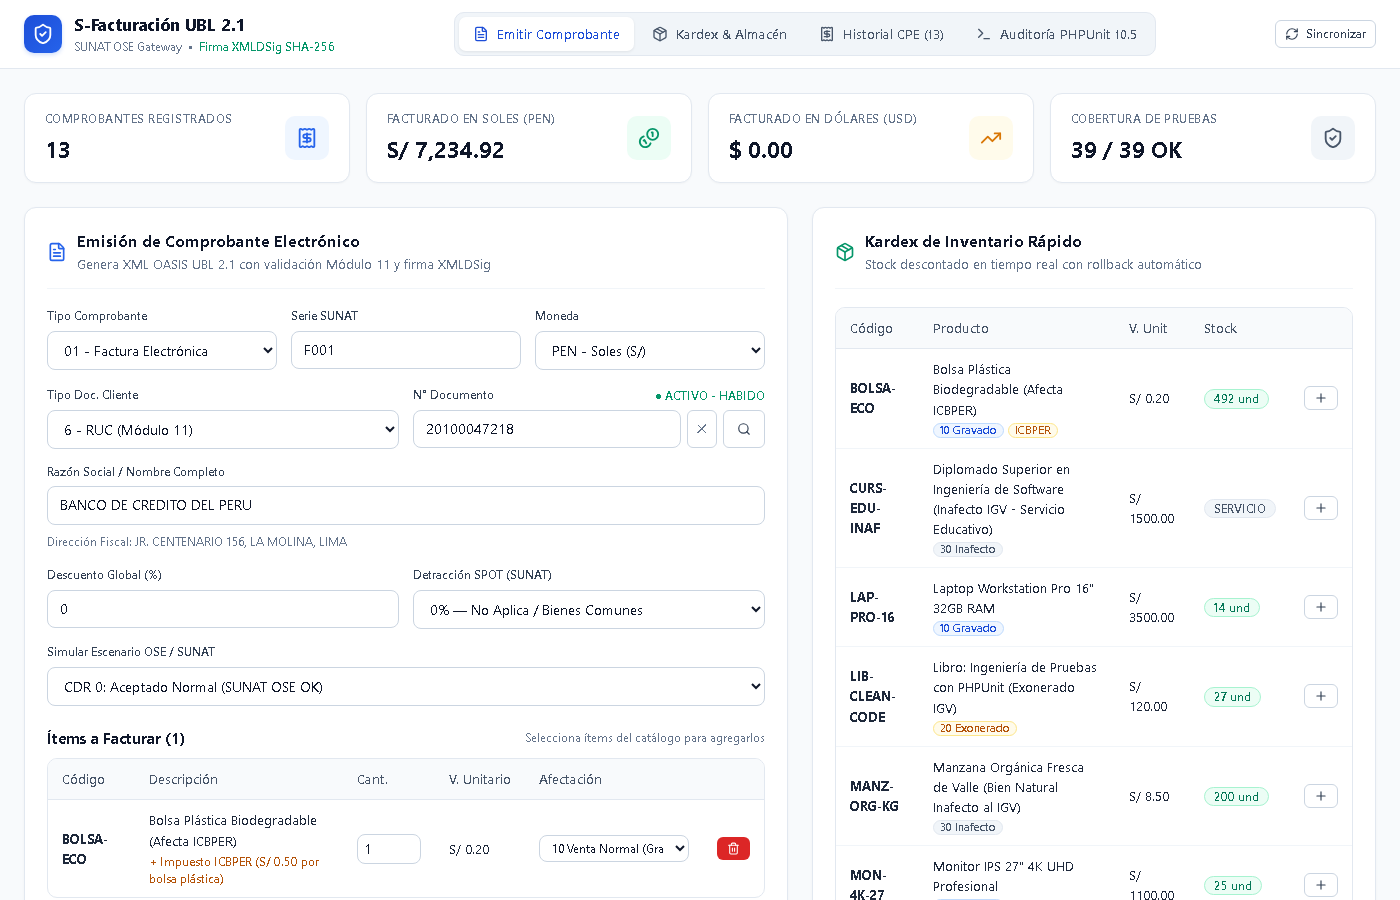
\includegraphics[width=0.96\textwidth,height=3.4cm,keepaspectratio]{capturas/01_app_facturador.png}\\[0.1cm]
        {\fontsize{6.2pt}{7.2pt}\selectfont\color{accentblue}\textbf{Figura 1:} Emisión en tiempo real en \texttt{localhost:5173}}
    \end{center}
\end{column}
\begin{column}{0.5\textwidth}
    \begin{center}
        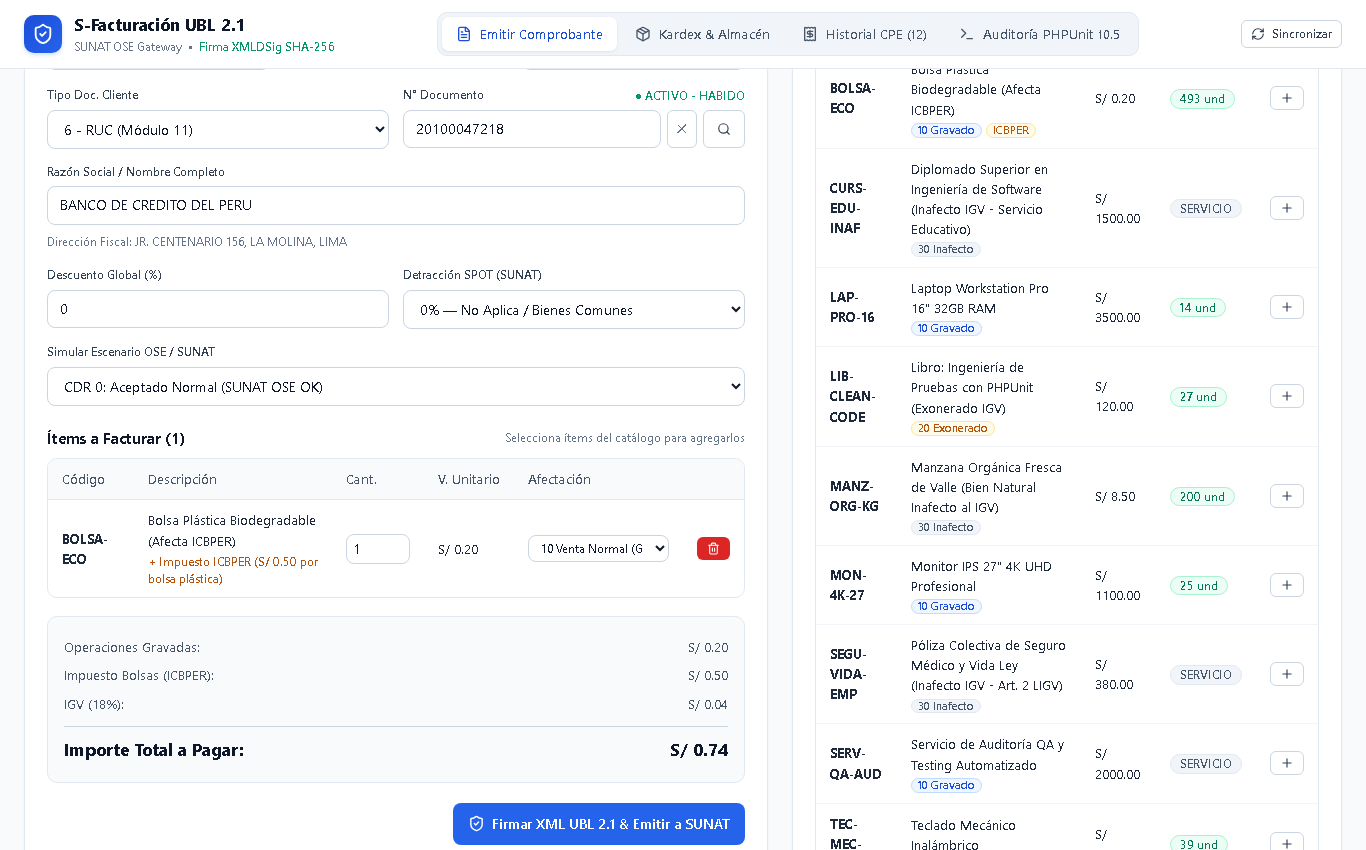
\includegraphics[width=0.96\textwidth,height=3.4cm,keepaspectratio]{capturas/02_catalogo_kardex_stock.png}\\[0.1cm]
        {\fontsize{6.2pt}{7.2pt}\selectfont\color{accentgreen}\textbf{Figura 2:} Catálogo de 9 productos y Kardex atómico}
    \end{center}
\end{column}
\end{columns}
\vspace{0.1cm}
{\fontsize{6pt}{7pt}\selectfont\color{textgray}\centering Ambas vistas validan la sincronización de inventario y el cálculo tributario con interfaz reactiva moderna.}
\end{frame}

% ==========================================
% SLIDE 18: EVIDENCIA EN VIVO: HISTORIAL Y VISOR XML (DIMENSIÓN AJUSTADA)
% ==========================================
\begin{frame}{17. Evidencias del Sistema en Ejecución: Historial y Visor UBL 2.1}
\begin{columns}
\begin{column}{0.5\textwidth}
    \begin{center}
        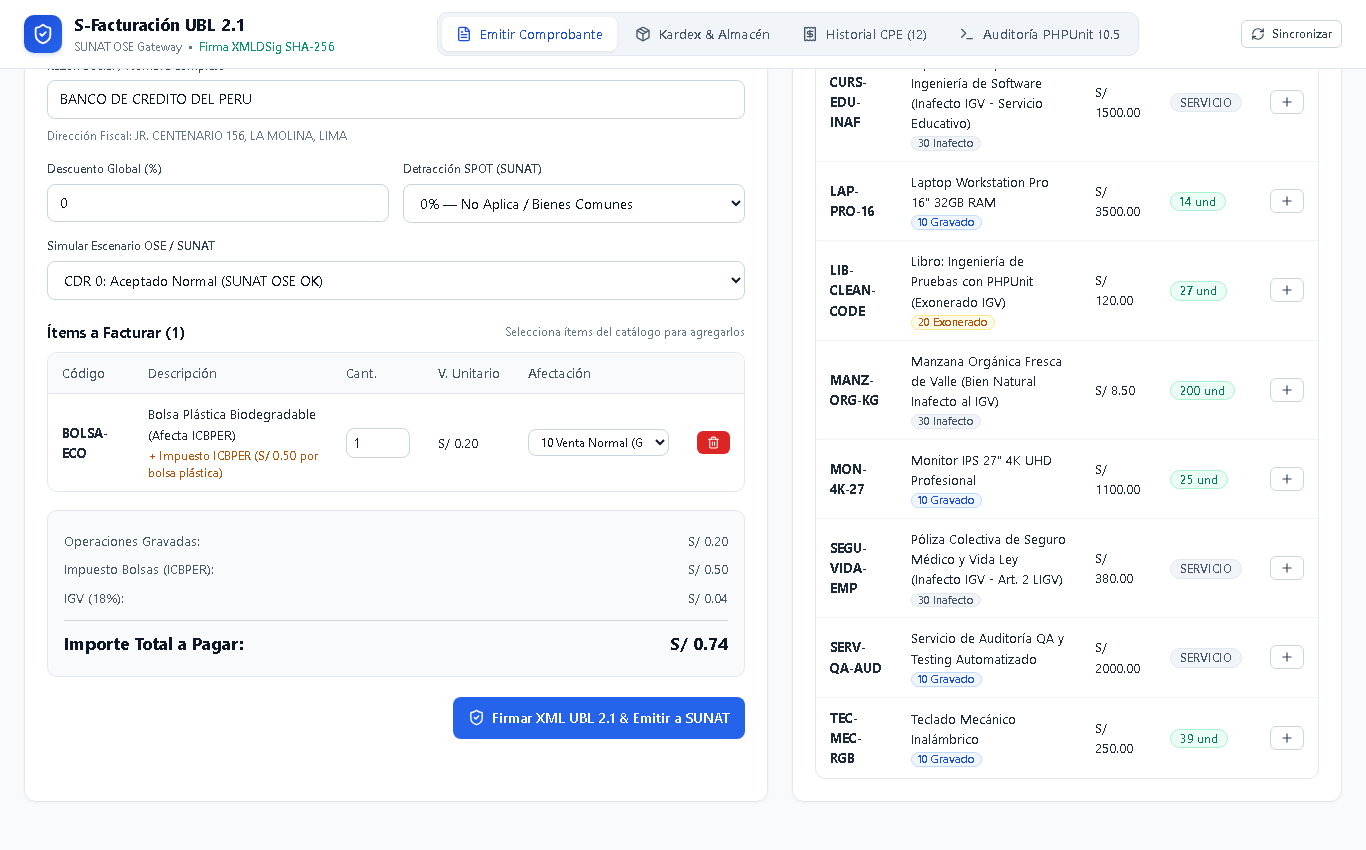
\includegraphics[width=0.96\textwidth,height=3.4cm,keepaspectratio]{capturas/03_historial_comprobantes_acciones.png}\\[0.1cm]
        {\fontsize{6.2pt}{7.2pt}\selectfont\color{accentblue}\textbf{Figura 3:} Bandeja fiscal con hash SHA-256}
    \end{center}
\end{column}
\begin{column}{0.5\textwidth}
    \begin{center}
        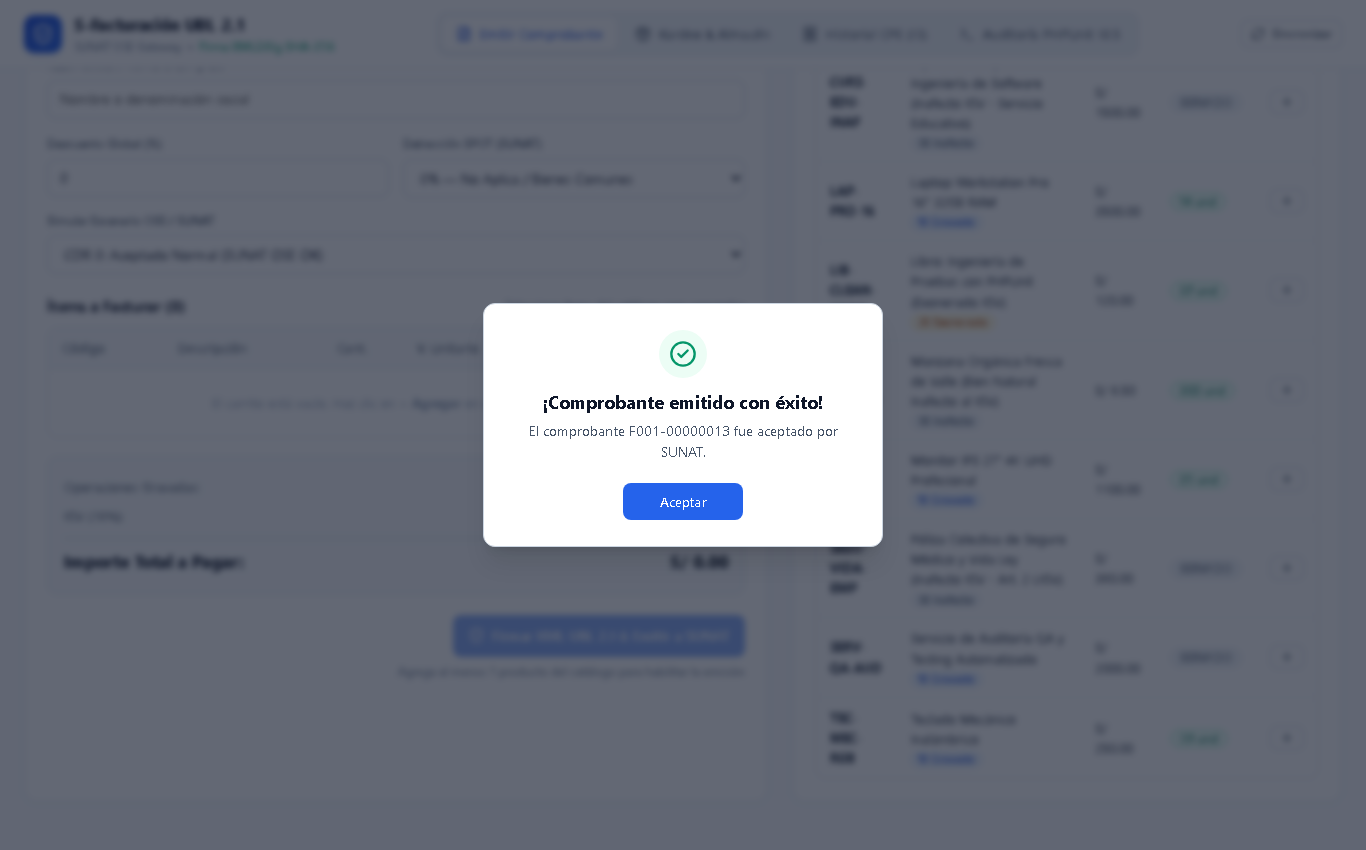
\includegraphics[width=0.96\textwidth,height=3.4cm,keepaspectratio]{capturas/04_visor_xml_ubl21.png}\\[0.1cm]
        {\fontsize{6.2pt}{7.2pt}\selectfont\color{accentgreen}\textbf{Figura 4:} Visor del XML estructurado con firma digital}
    \end{center}
\end{column}
\end{columns}
\vspace{0.1cm}
{\fontsize{6pt}{7pt}\selectfont\color{textgray}\centering Permite inspeccionar en vivo la firma digital XMLDSIG y descargar la constancia de recepción (CDR).}
\end{frame}

% ==========================================
% SLIDE 19: EVIDENCIA EN VIVO: TERMINAL PHPUNIT (DIMENSIÓN AJUSTADA)
% ==========================================
\begin{frame}{18. Evidencia Oficial: Salida Íntegra de Terminal PHPUnit 10.5}
\begin{center}
    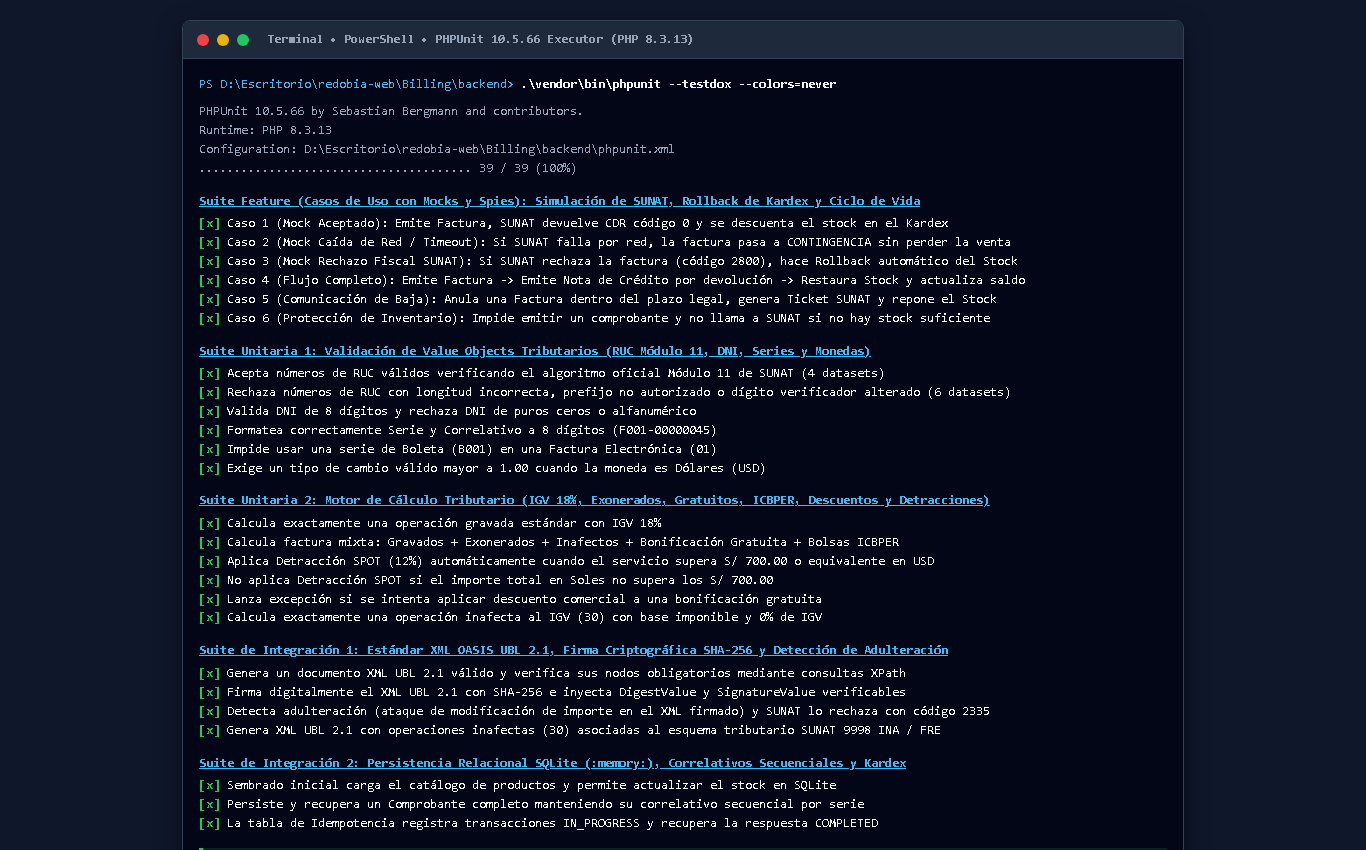
\includegraphics[width=0.88\textwidth,height=3.5cm,keepaspectratio]{capturas/07_terminal_phpunit_completo.png}\\[0.12cm]
    {\fontsize{7pt}{8pt}\selectfont\color{accentgreen}\textbf{Figura 5:} 39 Tests en Verde $\bullet$ 140 Aserciones Auditadas $\bullet$ 0.21 segundos en RAM}
\end{center}
\vspace{0.05cm}
{\fontsize{6pt}{7pt}\selectfont\color{textgray}\centering Ejecutado con \texttt{vendor/bin/phpunit --testdox --colors=never} cumpliendo el 100\% de las especificaciones.}
\end{frame}

% ==========================================
% SLIDE 20: CONCLUSIONES Y LECCIONES DE QA
% ==========================================
\begin{frame}{19. Conclusiones y Evaluación del Proceso de Calidad}
\begin{columns}
\begin{column}{0.5\textwidth}
    \begin{tcolorbox}[colback=cardbg, colframe=cardbg, title=\color{accentblue}\bfseries Conclusiones de Ingeniería de QA]
        \begin{itemize}
            \item \textbf{Arquitectura Hexagonal:} Desacoplar el Dominio de la Infraestructura permitió simular el 100\% de los escenarios fiscales sin depender de SUNAT.
            \item \textbf{Velocidad In-Memory (0.21s):} El uso de SQLite \texttt{:memory:} elimina la latencia de disco, incentivando correr los tests en cada commit.
            \item \textbf{Seguridad Criptográfica:} El Tamper Test demuestra inmunidad contra la alteración de montos en comprobantes UBL 2.1.
        \end{itemize}
    \end{tcolorbox}
\end{column}
\begin{column}{0.5\textwidth}
    \begin{tcolorbox}[colback=cardbg, colframe=cardbg, title=\color{accentgreen}\bfseries Certificación del Software]
        \begin{center}
            {\fontsize{10pt}{12pt}\selectfont\color{accentgreen}\bfseries 100\% COBERTURA CRÍTICA}\\[0.08cm]
            {\fontsize{6.8pt}{8pt}\selectfont\color{textwhite}39 de 39 Pruebas Aprobadas}\\[0.05cm]
            {\fontsize{6.8pt}{8pt}\selectfont\color{textwhite}140 de 140 Aserciones en Verde}\\[0.15cm]
            \rule{0.8\textwidth}{0.3pt}\\[0.15cm]
            {\fontsize{6pt}{7pt}\selectfont\color{textgray}
            Certificado bajo normativa SUNAT R.S. 097-2012\\
            y estándar internacional OASIS UBL 2.1
            }
        \end{center}
    \end{tcolorbox}
\end{column}
\end{columns}
\end{frame}

% ==========================================
% SLIDE 21: CIERRE Y PREGUNTAS
% ==========================================
\begin{frame}[plain]
\vspace{1.2cm}
\begin{center}
    {\fontsize{18pt}{22pt}\selectfont\bfseries\color{accentblue}¡Muchas Gracias!}\\[0.3cm]
    {\fontsize{10pt}{12pt}\selectfont\color{textwhite}Espacio para Ronda de Preguntas y Sustentación Técnica}\\[0.5cm]
    \begin{tcolorbox}[colback=cardbg, colframe=cardbg, width=0.82\textwidth, arc=2.5mm, boxrule=0mm]
        \begin{center}
        \fontsize{7pt}{8.5pt}\selectfont\color{textgray}
        Sistema de Facturación Electrónica UBL 2.1 $\bullet$ Automatización con PHPUnit 10.5\\[0.06cm]
        \color{accentamber}\textbf{Equipo de Calidad:} Apolinario, Umeres, Vasquez, Ventocilla\\[0.06cm]
        \color{accentblue}\texttt{github.com/fujimor1/Billing}
        \end{center}
    \end{tcolorbox}
\end{center}
\end{frame}

\end{document}
